% !TeX document-id = {2870843d-1baa-4f6a-bd0a-a5c796104a32}
% !BIB TS-program = biber
% !TeX encoding = UTF-8
% TU Delft beamer template

\documentclass[aspectratio=43]{beamer}
\usepackage[english]{babel}
\usepackage{csquotes}
\usepackage{calc}
\usepackage[absolute,overlay]{textpos}
\usepackage{graphicx}
\usepackage{subfig}
\usepackage{mathtools}
\usepackage{amsfonts}
\usepackage{amsthm}
\usepackage{comment}
\usepackage{siunitx}
\usepackage{MnSymbol,wasysym}
\usepackage{array}
\usepackage{qrcode}
\usepackage{hyperref}
\usepackage{physics}
\usepackage{tikz}
\usetikzlibrary{quantikz}

\setbeamertemplate{navigation symbols}{} % remove navigation symbols
\mode<presentation>{\usetheme[verticalbar=false]{tud}}

% BIB SETTINGS
\usepackage[
    backend=biber,
    giveninits=true,
    maxnames=30,
    maxcitenames=20,
    uniquename=init,
    url=false,
    style=authoryear,
]{biblatex}
\addbibresource{bibfile.bib}
\setlength\bibitemsep{0.3cm} % space between entries in the reference list
\renewcommand{\bibfont}{\normalfont\scriptsize}
\setbeamerfont{footnote}{size=\tiny}
\renewcommand{\cite}[1]{\footnote<.->[frame]{\fullcite{#1}}}
\setlength{\TPHorizModule}{\paperwidth}
\setlength{\TPVertModule}{\paperheight}

\newcommand{\absimage}[4][0.5,0.5]{%
	\begin{textblock}{#3}%width
		[#1]% alignment anchor within image (centered by default)
		(#2)% position on the page (origin is top left)
		\includegraphics[width=#3\paperwidth]{#4}%
\end{textblock}}

\newcommand{\mininomen}[2][1]{{\let\thefootnote\relax%
	\footnotetext{\begin{tabular}{*{#1}{@{\!}>{\centering\arraybackslash}p{1em}@{\;}p{\textwidth/#1-2em}}}%
	#2\end{tabular}}}}

% New commands (Giorgio)
\newcommand{\R}{\mathbb{R}}  % real set
% \newcommand{\pdv}[2]{\frac{\partial #1}{\partial #2}}
\newcommand{\inner}[2]{\langle #1,\, #2\rangle}
\newcommand{\kernel}[2]{\kappa\left( #1, #2 \right)}

\DeclarePairedDelimiter\ceil{\lceil}{\rceil}
\DeclarePairedDelimiter\floor{\lfloor}{\rfloor}


\title[]{Applied Quantum Algorithms - Lecture 9 - Quantum Kernel Methods}
\institute[]{Delft University of Technology, The Netherlands}
\author{Giorgio Tosti Balducci}
\date{May 3, 2023}


\begin{document}
\section{Introduction}
{
\setbeamertemplate{footline}{\usebeamertemplate*{minimal footline}}
\frame{\titlepage}
}

\begin{frame}{Contents} % some commands, e.g. \verb require [fragile]
\begin{enumerate}
  \item Learning with quantum kernels
  \begin{enumerate}
    \item Quantum supervised ML models are kernel methods\cite{Schuld_2021_kernels}
    \item Support Vector Machines (SVMs)
    \item Comparing quantum kernels and variational QC models
    % \item Choosing the right kernel
  \end{enumerate}
  \item Demo
\end{enumerate}
\end{frame}

\section{Lecture}

\begin{frame}
  \frametitle{The density matrix representation of quantum states}
  \small
  We're used to represent quantum states as
  \[\ket{\psi} = \psi_0\ket{0\dots 0} + \psi_{2^n-1}\ket{1\dots 1}\] 

  \ \\
  \pause
  But there exist an alternative representation as \emph{density matrices}
  \[\rho = \ketbra{\psi}{\psi}\]

  \ \\
  Generally speaking, the usefullness of density matrices is in describing \emph{mixed states}, i.e. probabilistic quantum states
  \[\rho = \sum p_i \ketbra{\psi^{(i)}}{\psi^{(i)}}\]

  \ \\
  \pause
  However, what's important for us is that \emph{quantum kernel theory} uses the density matrix formalism
  \begin{itemize}
    \item<4-> As we shall see, this is because quantum models are linear in the data mapped as density matrices, but not as ket vectors.
    \item<5-> With this premise, forget about the name `matrix' and just think to the $\rho$-space as a \emph{vector space}.
  \end{itemize}
\end{frame}


\begin{frame}
  \frametitle{Data encoding as a feature map in the $\rho(x)$ space}

  Given
  \[\mathcal{F} = \left\{ \rho \in \mathbb{C}^{2^n\times 2^n} \right\},\]

  we define data encoding as a map
  \[\phi:\mathcal{X}\rightarrow \mathcal{F}, \qquad \phi(\mathbf{x}) = \ketbra{\phi(\mathbf{x})} = \rho\left( \mathbf{x} \right).\]

  \ \\
  \pause
  $\mathcal{F}$ has an \emph{inner product} defined and it's therefore a \emph{Hilbert space}
  \[\inner{\rho}{\sigma}_\mathcal{F} = \tr\left[ \rho \sigma \right]\]
  
\end{frame}


\begin{frame}
  \frametitle{Data encoding as a feature map in the $\rho(x)$ space}
  \framesubtitle{Operatively}

  Recall
  \begin{center}
    \begin{quantikz}
      \lstick[4]{$\ket{0}^n$} &\gate[4]{U(\mathbf{x})} & \gate[4]{W(\mathbf{\theta})^\dagger} & \meter{}\\
      & & & \meter{}  \\
      & & & \meter{}  \\
      & & & \meter{} 
    \end{quantikz}
\end{center}

  \ \\
  \pause
  $U(\mathbf{x})$ is what implements $\phi\left( \mathbf{x} \right)$

\end{frame}


\begin{frame}
  \frametitle{Quantum kernels}
  \framesubtitle{Inner products of quantum feature vectors}

  As we've seen, a feature map of data to a Hilbert space induces a \emph{new metric of distance}
  \begin{itemize}
    \item<2-> a.k.a. inner product in $\mathcal{F}$
    \item<3-> a.k.a. \emph{kernel}
    \onslide<3->{\[\kappa:\mathcal{X}\times\mathcal{X} \rightarrow \R\]}
  \end{itemize}

  \ \\
  \onslide<4>{
  When $\mathcal{F}$ is the space of density matrices
  \[\kernel{\mathbf{x}}{\mathbf{x}^\prime} = \tr\left[ \rho\left( \mathbf{x} \right) \rho\left( \mathbf{x}^\prime \right) \right] = \abs{\ip{\phi(\mathbf{x})}{\phi(\mathbf{x}^\prime)}}^2\]
  }

\end{frame}


\begin{frame}
  \frametitle{Quantum kernels}
  \framesubtitle{Kernels induced by the data encodings we know}

  \begin{table}[htbp]
    \centering\begin{tabular}{ll}
      Encoding & Kernel \\
      \hline \\
      Basis encoding & $\delta_{\mathbf{x},\mathbf{x}^\prime}$\\
      Amplitude encoding & $\abs{\mathbf{x}^\dagger \mathbf{x}^\prime}^2$\\
      Repeated amplitude encoding & $(\abs{\mathbf{x}^\dagger \mathbf{x}^\prime}^2)^r$\\
      Angle encoding & $\prod_{k=1}^N\cos(\mathbf{x}_k-\mathbf{x}_k^\prime)$\\
      General time-evolution encoding & $\sum_{\mathbf{s},\mathbf{t}\in\Omega}c_{\mathbf{s},\mathbf{t}}e^{i\mathbf{s}^T\mathbf{x}}e^{i\mathbf{t}^T\mathbf{x^\prime}}$\\
      \hline
    \end{tabular}
  \end{table}

  \ \\
  \pause
  \footnotesize
  Also, if we map data to a photonic circuit, we map to the infinite dimensional basis of Fock states. Interestingly, it's easy to show that the kernel of this feature map is a \emph{Gaussian kernel}
  \[\kappa(\mathbf{x}, \mathbf{x}^\prime)=e^{-\abs{\mathbf{x}-\mathbf{x}^\prime}^2}\]

\end{frame}


\begin{frame}
  \frametitle{Quantum kernels}
  \framesubtitle{Question 1}

  \centering
  \textcolor{red}{What does the kernel expression for \emph{basis encoding} tell us about how we can learn with it?}
  
  \ \\
  \emph{Tip:} think about classification

\end{frame}


\begin{frame}
  \frametitle{Quantum kernels}
  \framesubtitle{Question 2}

  \centering
  \color{red} Is (repeated) amplitude encoding the same as the classical polynomial encoding?

\end{frame}


\begin{frame}
  \frametitle{Back to quantum models}

  In lecture 8, we defined the supervised QML model as
  \[f(\mathbf{x}, \theta) = \ev{\mathcal{M}}{\psi\left( \mathbf{x}, \theta \right)},\]

  where
  \[\ket{\psi\left( \mathbf{x}, \theta \right)} = W\left( \theta \right) U(\mathbf{x}) \ket{0}.\]

  \pause
  In density matrix representation
  \[f(\mathbf{x}, \theta) = \tr\left[ \ketbra{\psi\left( \mathbf{x},\theta \right)}\mathcal{M} \right] = \tr\left[\rho\left( \mathbf{x},\theta \right)\mathcal{M}\right]\]

  \pause
  The parameters $\theta$ can be included in $\mathcal{M}_\theta$ (objective: find the optimal measurement). For the time being, however let's forget about them
  \[f(\mathbf{x})=\tr\left[\rho\left( \mathbf{x} \right)\mathcal{M}\right]\]

  \pause
  In this way, \emph{our models are measurements in feature space}.

\end{frame}


\begin{frame}
  \frametitle{What Hilbert spaces are associated to a QML model?}

  \begin{enumerate}
    \item Feature space: $\mathcal{F}=\left\{ \phi:\mathcal{X}\rightarrow \mathbb{C}^{4n}| \phi:\mathbf{x}\rightarrow \rho\left( \mathbf{x} \right) \right\}$
    \item Space of quantum models: $\left\{ f:\mathcal{X}\rightarrow\R| f\left( \mathbf{x} \right)=\tr\left[ \rho\left( \mathbf{x} \right)\mathcal{M} \right] \right\}$
  \end{enumerate}

  \ \\
  What is the relation between the two?
  \pause
  \begin{block}{Theorem 1}
    Quantum models of the form $\tr\left[\rho\left( \mathbf{x} \right)\mathcal{M}\right]$ are linear models in the feature vectors $\rho\left( \mathbf{x} \right)\in \mathcal{F}$.
    \note{proof on whiteboard}
  \end{block}

  \pause
  \begin{block}{Theorem 2}
    Measurements in feature space are linear combination of feature vectors
    \[\mathcal{M} = \sum_i \gamma_i \rho\left( \mathbf{x}^{(i)} \right)\]
    \note{proof on whiteboard}
  \end{block}

\end{frame}


\begin{frame}
  \frametitle{A Hilbert space induced by the kernel}
  \framesubtitle{The Reproducing Kernel Hilbert Space (RKHS)}
  \pause
  Let's forget about quantum models for a moment and let's focus on \emph{kernels}. We can define a \emph{Hilbert space} $F$ induced by $\kappa\left( \mathbf{x}, \cdot \right)$

  \pause
  \begin{exampleblock}{Reproducing Kernel Hilbert Space (RKHS)}
    The Hilbert space $F$ that is the span of the functions $g(\cdot)=\kappa\left( \mathbf{x}, \cdot\right)$ and where the inner product between $g(\cdot)=\sum_i \alpha_i \kappa\left( \mathbf{x}^{(i)}, \cdot\right)$ and $h(\cdot)=\sum_i \beta_i \kappa\left( \mathbf{x}^{(i)}, \cdot\right)$ is

    \[\inner{g}{h}_F = \sum_{i,j} \alpha_i \beta_j \kappa\left( \mathbf{x}_i, \mathbf{x}_j \right)\]
  \end{exampleblock}

  \ \\
  \pause
  A bit more intuitively:
  \begin{itemize}
    \item The RKHS is the space that associates each data point with a \emph{function}, which is its distance measure (inner product) in feature space.
  \end{itemize}
  
\end{frame}


\begin{frame}
  \frametitle{RKHS}
  \framesubtitle{Intuition}

  Gaussian kernel: $\kernel{\mathbf{x}}{\mathbf{x}^\prime} = e^{-\frac{\gamma}{2}\abs{\mathbf{x}-\mathbf{x}^\prime}^2}$

  \ \\
  \centering
  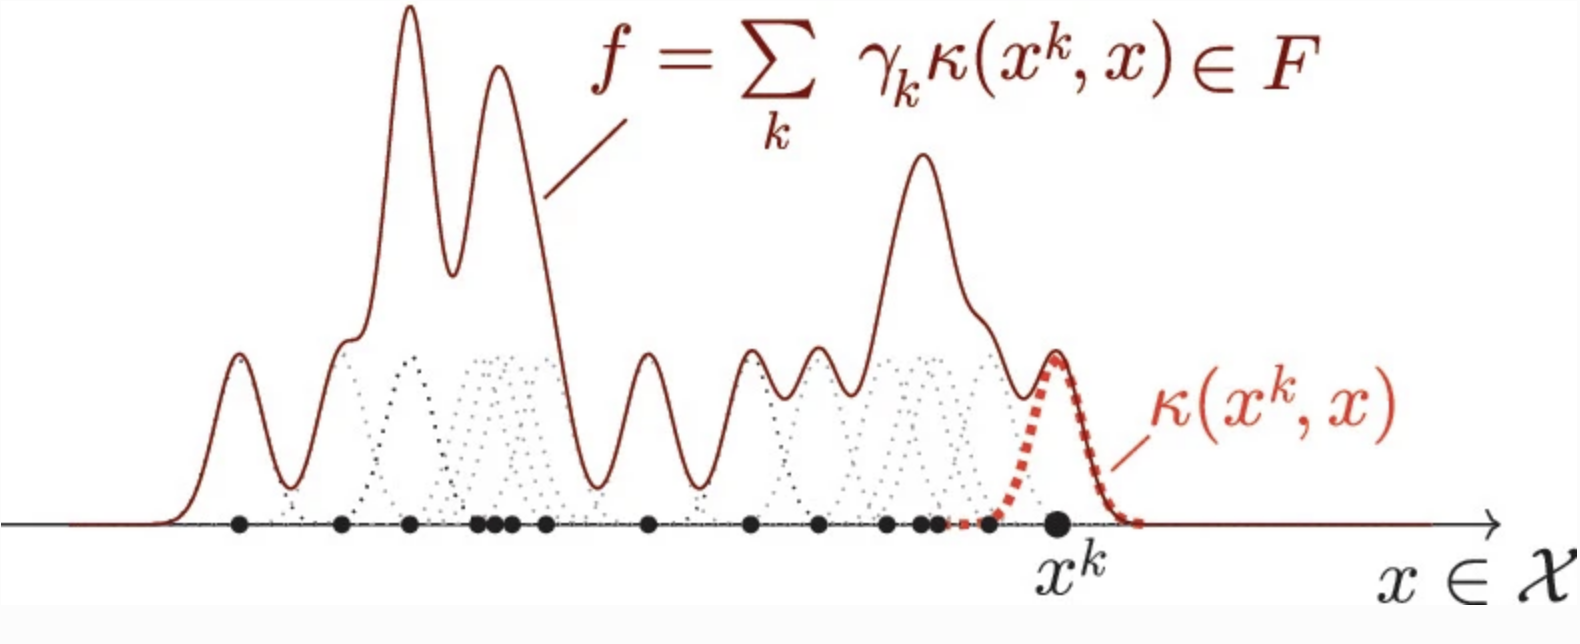
\includegraphics[width=.5\textwidth]{pics/schuld-rkhs-intuitive.png}

  By tuning $\gamma$, we tune how each point $\mathbf{x}\in \mathcal{X}$ `affects' (is similar to) each other.

\end{frame}


\begin{frame}
  \frametitle{RKHS}
  \framesubtitle{Why do we care?}

  \pause
  \begin{block}{Theorem 3}
    Functions in the RKHS $F$ are linear models in the data-encoding features in $\mathcal{F}$ and vice-versa.

    \begin{itemize}
      \item The RKHS is the same as the space of quantum models!
    \end{itemize}
  \end{block}

  \ \\
  \pause
  Therefore, if we can prove something about the RKHS induced by $\kappa\left( \mathbf{x}, \mathbf{x}^\prime\right)$, the same property holds for our quantum model $\tr[\rho\left( \mathbf{x} \right)\mathcal{M}]$.
  \begin{itemize}
    \item universality
    \item trainability
    \item generalization
  \end{itemize}

\end{frame}


\begin{frame}
  \frametitle{The vector spaces of quantum models}

  \centering
  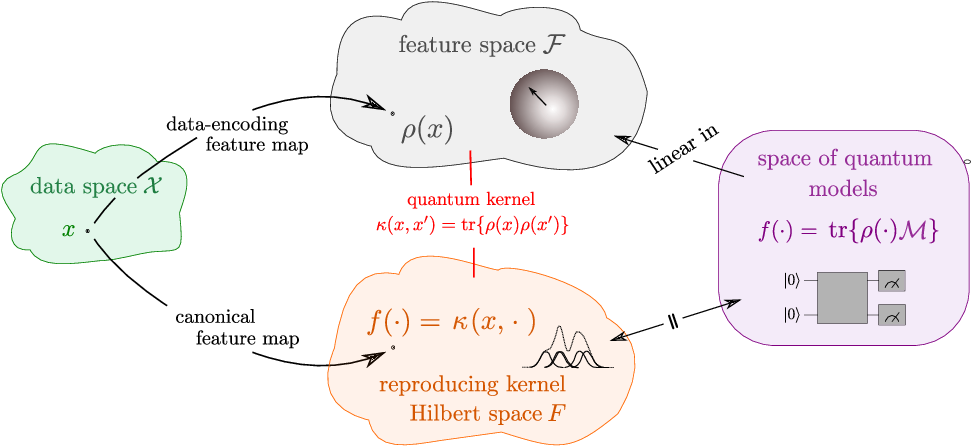
\includegraphics[width=\textwidth]{pics/schuld-overview.png}

\end{frame}


\begin{frame}
  \frametitle{Training with kernels}
  \framesubtitle{The representer theorem}

  \small
  \begin{itemize}
    \item<1-> The RKHS corresponds to the space of linear models in $\mathcal{F}$
    \item<2-> Then we can search for the \emph{optimal model} directly in the RKHS
    \item<3-> For optimal model we mean the one that minimizes the \emph{regularized empirical risk}
    \[f_{\mathrm{opt}} = \mathrm{argmin}_{f\in F}\left\{ \hat{\mathcal{R}}\left( f \right) + g\left( \norm{f} \right)_F \right\},\]
    where
    \[\hat{\mathcal{R}}\left( f \right) = \frac{1}{M}\sum_{m=1}^M L\left( \mathbf{x}^{(m)}, y^{(m)}, f(\mathbf{x}^{(m)}) \right)\]
  \end{itemize}

  \pause
  \begin{block}{Theorem 4: \emph{Representer theorem}}
    Given a dataset $\mathcal{D}=\left\{ \left( \mathbf{x}^{(0)}, y^{(0)} \right), \dots, \left( \mathbf{x}^{(M-1)}, y^{(M-1)} \right) \right\}$, the $f\in \mathcal{F}$ that minimizes the empirical risk is a linear combination of $f\in \mathcal{F}$ centered in the datapoints, i.e.
    \[f_{\mathrm{opt}}=\sum_{m=0}^{M-1} c_m f_{\mathbf{x}^{(m)}} = \sum_{m=0}^{M-1} c_m \kernel{\mathbf{x}^{(m)}}{\mathbf{x}}\]
  \end{block}
  

\end{frame}


\begin{frame}
  \frametitle{Training with kernels}
  \framesubtitle{The representer theorem}
  
  \footnotesize
  \begin{block}{Corollary for quantum models: \emph{optimal measurement}}
    The measurement in $\mathcal{F}$ that minimizes the empirical risk is a linear expansion of the feature vectors of the data-points
    \[\mathcal{M}_{\mathrm{opt}} = \sum_{m=0}^{M-1} c_m \rho\left( \mathbf{x}^{(m)} \right)\]
  \end{block}

  \pause
  Consequences
  \begin{itemize}
    \item<2-> Optimizing any kernel-based model is at most a $M$-dimensional optimization problem.
    \item<3-> For algorithms s.a. \emph{support vector machines} (SVMs), the data-points that `support' the optimal model are generally even less.
    \begin{itemize}
      \item More soon\dots
    \end{itemize}
    \item<4-> Given a feature map (a.k.a. data encoding in quantum), \emph{we are ensured that the optimal model lives in the space spanned by linear models in feature spaces} (i.e. kernel-based models)
    \begin{itemize}
      \item Often reachable with \emph{convex optimization}
      \item More soon\dots
    \end{itemize}
  \end{itemize}

\end{frame}


\begin{frame}
  \frametitle{A note on regularization}

  What is exactly $\norm{f}_F$? How do we \emph{operatively} compute norms in the RKHS?

  \ \\
  \pause
  It turns out that
  \begin{itemize}
    \item<2-> Not only $\kernel{\mathbf{x}}{\cdot}$ builds the space where the model with minimum reg. emp. risk lives
    \item<2-> It also defines a transformation $\Gamma:F\rightarrow L_2(\mathcal{X})$ from the RKHS to the square integrable function space, such that
    \[\inner{f}{f}_F=\inner{\Gamma f}{\Gamma f}_{L_2} = \int_\mathcal{X} \left( \Gamma f(\mathbf{x})  \right)^2 \mathrm{d}\mathbf{x}\]
    \item<3-> Which allows us to compute $\inner{f}{f}_F$
    \begin{itemize}
      \item we know which quantity of $f$ we penalize during regularization.
    \end{itemize} 
  \end{itemize}

  \onslide<3->{
  \emph{Note}: each kernel induces a different RKHS and a different $\Gamma$
  }
\end{frame}


\begin{frame}
  \frametitle{Kernel-based optimization}

  Kernel theory also gives us guarantees about optimization

  \pause
  \begin{block}{Theorem 5}
    The problem of finding the kernel-based model that minimizes the regularized empirical risk is finite-dimensional and it is convex if the loss function is convex.
  \end{block}

  \pause
  \footnotesize
  The proof for quantum kernels is easy: by substituting 
  \[f_{\mathrm{opt}}\left( \mathbf{x} \right) = \sum_m c_m \tr\left[ \rho\left( \mathbf{x}^{(m)} \right) \rho\left( \mathbf{x} \right)\right]\]
  into
  \[\mathrm{argmin}_{f\in F}\left\{ \hat{\mathcal{R}}\left( f \right) + \lambda \norm{f}^2_F \right\},\]
  we obtain
  \[\mathrm{argmin}_\mathbf{c} \frac{1}{M}\sum_m L\left( x^{(m)}, y^{(m)}, \sum_{m^\prime} c_{m^\prime} \kernel{\mathbf{x}^{(m)}}{\mathbf{x}^{(m^\prime)}} \right) + \lambda \mathbf{c}^\top \mathbf{K} \mathbf{c},\]
  which is a convex optimization problem if $L$ is convex.

\end{frame}


\begin{frame}
  \frametitle{Kernel-based optimization}

  \begin{itemize}
    \item<1-> We know $O(M^2)$-time algorithms that can solve convex optimization
    \item<2-> With fault-tolerant quantum computing, we can even reduce this to $O(M)$
    \item<3-> We are guaranteed to find the global optimum
  \end{itemize}

  \ \\
  \onslide<4->{
  Now that we know all about kernel theory\dots
  \begin{itemize}
    \item<5-> What actual ML algorithms use kernels?
    \begin{itemize}
      \item<6-> We will see one of them, \emph{support vector machines} in which kernels appear naturally in writing the optimization problem\footnote{Note that SVM can also be obtained by plugging the \emph{hinge loss} (convex) into the regularized empirical risk seen in the previous slide.}.
    \end{itemize} 
    \item<7-> But first\dots
  \end{itemize}
  }

\end{frame}


\begin{frame}
  \frametitle{Quantum kernel circuits}
  \framesubtitle{How do we compute kernels on quantum hardware?}

  \pause
  \begin{center}
    \begin{quantikz}
      \lstick[4]{$\ket{0}^n$} &\gate[4]{U(\mathbf{x}^{(i)})} & \gate[4]{U(\mathbf{x}^{(j)})^\dagger} & \meter{} & \rstick[4]{$p\left( \ket{0}^n \right)$}\\
      & & & \meter{} &  \\
      & & & \meter{} &  \\
      & & & \meter{} & 
    \end{quantikz}
  \end{center}

  \pause
  \small
  Intuition:
  \begin{itemize}
    \item<3-> if $U(\mathbf{x}^{(i)})\ket{0}^n \approx U(\mathbf{x}^{(j)})\ket{0}^n$, then $p\left( \ket{0}^n \right) \approx 1$
    \begin{itemize}
      \item<3-> and if $\mathbf{x}^{(i)} = \mathbf{x}^{(j)}$, then $p\left( \ket{0}^n \right) = 1$
    \end{itemize}
    \item<4-> else, $p\left( \ket{0}^n \right) \neq 1$ or even $p\left( \ket{0}^n \right) = 0$ ($\mathbf{x}^{(i)},\, \mathbf{x}^{(j)}$ are orthogonal in feature space)
  \end{itemize}


\end{frame}


\begin{frame}
  \frametitle{Quantum kernel circuits}

  \centering
  \color{red} In binary classification, should our quantum $\kernel{\mathbf{x}^{(i)}}{\mathbf{x}^{(i)}}$ give us highly-spaced probabilities or a (maybe uniform) range of probabilities?

\end{frame}


\begin{frame}
  \frametitle{Support vector machines}

  \begin{columns}[onlytextwidth]
    \begin{column}{.5\textwidth}
      \centering
      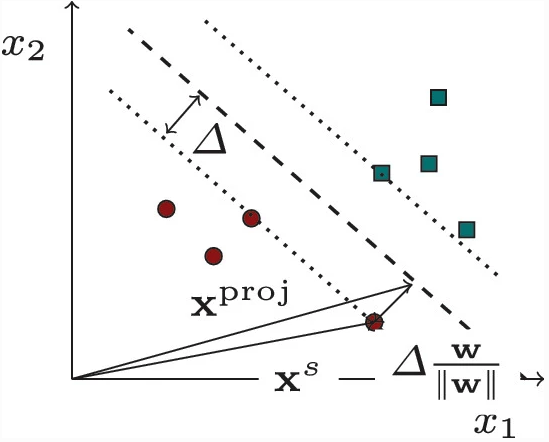
\includegraphics[width=\textwidth]{pics/supp-vecs.png}
      \[\mathcal{X} \subset \R^N,\: \mathcal{Y} = \left\{ -1,1 \right\}^N\]
    \end{column}
    \begin{column}{.5\textwidth}
      \small
      \begin{itemize}
        \item<2-> Assume linear separability (will be relaxed later)
        \item<3-> There exists a hyperplane with normal $\mathbf{w}$ and bias $b$
        \[f_\mathbf{w}(\mathbf{x}) = \mathbf{w}^\top \mathbf{x} + b\]
        \item<4-> Because of linear separability
      \[f\left( \mathbf{x}^{(m)} \right)y^{(m)} > 0\] 
      \end{itemize}
    \end{column}
  \end{columns}

\end{frame}


\begin{frame}
  \frametitle{Support vector machines}

  \begin{columns}[onlytextwidth]
    \begin{column}{.5\textwidth}
      \centering
      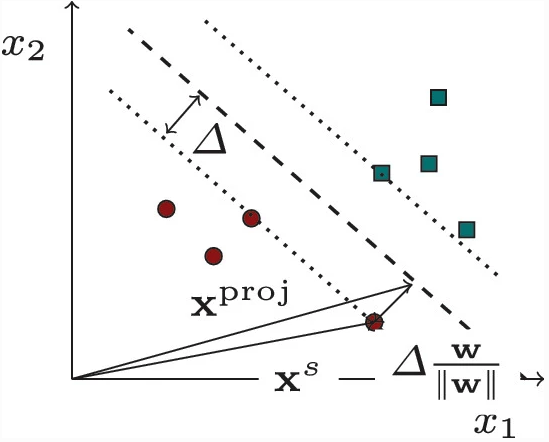
\includegraphics[width=\textwidth]{pics/supp-vecs.png}
      \[\mathcal{X} \subset \R^N,\: \mathcal{Y} = \left\{ -1,1 \right\}^N\]
    \end{column}
    \begin{column}{.5\textwidth}
      \small
      The objective in SVMs is to find the hyperplane that maximizes the \emph{margin}, i.e. the distance from the hyperplane the closest points (\emph{support vectors})
      \begin{itemize}
        \item<2-> Support vectors
        \[\mathbf{x}_s = \mathbf{x}_\mathrm{proj} + \Delta \frac{\mathbf{w}}{\norm{\mathbf{w}}}\]
        \item<3-> Substitute in the hyperplane's equation
        \[f\left( \mathbf{x}_s \right)=\mathbf{w}^\top\mathbf{x}_\mathrm{proj} + \Delta\norm{\mathbf{w}}\]
        \item<4-> Since $\mathbf{w}^\top\mathbf{x}_\mathrm{proj}=0$, we find the margin to be
        \[\Delta = \frac{f\left( \mathbf{x}_s \right)}{\norm{\mathbf{w}}}\]
      \end{itemize}
    \end{column}
\end{columns}

\end{frame}


\begin{frame}
  \frametitle{Support vector machines}
  \framesubtitle{Primal optimization problem}

  Now we're ready to define the SVM optimization problem\footnote{Formally, the problem is not well defined yet, because the length of $\mathbf{{w}}$ is not restricted. Therefore we add the additional condition that $\Delta \norm{\mathbf{w}}=1$}
  \pause
  \begin{align*}
    \mathrm{minimize}& \quad\frac{1}{2}\norm{w}^2,\\
    \mathrm{s.t.}& \quad y^{\left( m \right)}\left( \mathbf{w}^\top \mathbf{x}^{(m)} + b\right) > 0, \quad m={0,\dots, M-1},
  \end{align*}
  which is a \emph{quadratic convex optimization problem} in $N$ \emph{dimensions}.

  \ \\
  \pause
  We can also write the Lagrangian of the problem
  \[\mathcal{L}_{\mathrm{primal}}\left( \mathbf{w}, b, \mathbf{\alpha} \right) = \frac{1}{2}\norm{w}^2 + \sum_{m=0}^{M-1} \alpha_m y^{\left( m \right)}\left( \mathbf{w}^\top \mathbf{x}^{(m)} + b\right) \]

\end{frame}


\begin{frame}
  \frametitle{Support vector machines}
  \framesubtitle{Dual optimization problem}

  2 caveats
  \begin{itemize}
    \item<2-> The primal form is hard to translate to the \emph{nonlinearly separable case}.
    \item<3-> For high-dimensional data ($N \gg 1$), the problem of finding $N$ components of $\mathbf{w}$ gets expensive.
  \end{itemize}

  \onslide<4->{
  Can we rewrite the problem only in terms of $\alpha_m$?}
  \onslide<5->{
  \[\pdv{\mathcal{L}}{\mathbf{w}}=0 \rightarrow \mathbf{w} = \sum_{m=0}^{M-1} \alpha_m y^{(m)}\mathbf{x}^{(m)}\]
  \[\pdv{\mathcal{L}}{b}=0 \rightarrow b = \sum_{m=0}^{M-1} \alpha_m y^{(m)}\]
  }
\end{frame}


\begin{frame}
  \frametitle{Support vector machines}
  \framesubtitle{Dual optimization problem}

  By plugging the expressions of $\mathbf{w}$ and $b$ into the Lagrangian, we get
  \[\mathcal{L}_{\mathrm{dual}}\left( \mathbf{\alpha} \right) = \sum_{m=0}^{M-1}\alpha_m - \frac{1}{2}\sum_{m,m^\prime=0}^{M-1}\alpha_m\alpha_{m^\prime}y^{(m)}y^{(m^\prime)}\left( \mathbf{x}^{(m)} \right)^\top \mathbf{x}^{(m^\prime)}\]

  \begin{itemize}
    \item<2-> We still have a quadratic convex optimization problem (in the $\alpha_m$)
    \item<3-> $\alpha_m$ determine $\mathbf{w}$ and $b$
    \begin{itemize}
      \item<4-> The problem is now $M$-dimensional (number of samples)
      \item<5-> It turns out that $\alpha_m=0$, \emph{except at the support vectors}\footnote{More formally, this comes from the fact that the dual problem satisfies the Kush, Kuhn, Tucker (KKT) conditions}
      \begin{itemize}
        \item Intuitively, only the points close to the class boundary define the hyperplane
      \end{itemize}
    \end{itemize}
  \end{itemize}

\end{frame}


\begin{frame}
  \frametitle{Support vector machines}
  \framesubtitle{Dual optimization problem}
  
  But let's look to the dual Lagrangian a bit more\dots

  \[\mathcal{L}_{\mathrm{dual}}\left( \mathbf{\alpha} \right) = \sum_{m=0}^{M-1}\alpha_m - \frac{1}{2}\sum_{m,m^\prime=0}^{M-1}\alpha_m\alpha_{m^\prime}y^{(m)}y^{(m^\prime)}\left( \mathbf{x}^{(m)} \right)^\top \mathbf{x}^{(m^\prime)}\]

  \ \\
  \pause
  \begin{center}
    \textcolor{red}{Is there anything that suggests us an extension to the non-linearly separable case?}

    \pause
    \emph{Tip}: think to kernels
  \end{center}

  
\end{frame}


\begin{frame}
  \frametitle{Support vector machines}
  \framesubtitle{Dual optimization problem}
  
  \[\mathbf{x} \rightarrow \phi\left( \mathbf{x} \right) \quad \text{(feature map)}\]
  \pause
  \[\left( \mathbf{x}^{(m)} \right)^\top \mathbf{x}^{(m^\prime)} \rightarrow \inner{\phi\left( \mathbf{x}^{(m)} \right)}{\phi\left( \mathbf{x}^{(m^\prime)} \right)} = \kernel{\mathbf{x}^{(m)}}{\mathbf{x}^{(m^\prime)}}\]

  \ \\
  \pause
  Thanks to the inner product structure of the dual SVM, we can plug-in a kernel in place of $\left( \mathbf{x}^{(m)} \right)^\top \mathbf{x}^{(m^\prime)}$ and we can deal with non-linear separability.
  \begin{itemize}
    \item<4-> Provided that the feature map $\phi$ leads to linear separability in feature space.
  \end{itemize}
  

\end{frame}

% \section{Conclusion}
% \begin{frame}[fragile]{animation}
%   \vfill
%   Some commands take optional arguments in the form of \verb|<x-y>|,
%   where \verb|x| is the first `sub-frame' on which the context is shown,
%   and \verb|y| is the last. \verb|x| or \verb|y| can be replaced by \verb|+|,
%   referring to `the next sub-frame'. 
%   \vfill
%   \begin{columns}[onlytextwidth]
%   \begin{column}{.5\textwidth}
%     \begin{enumerate}
%       \item<+-> uncovered\ldots
%       \item<+-> one\ldots
%       \item<+-> by\ldots
%       \item<+-> one.
%     \end{enumerate}
%     \end{column}
%   \begin{column}{.5\textwidth}
%       Using only:\only<1>{1}\only<2>{2}\only<3>{3}

%       Using onslide:\onslide<1>{1}\onslide<2>{2}\onslide<3>{3}

%       Using pause:\pause1\pause2\pause3
%   \end{column}
%   \end{columns}
%   \vfill
%   For more advanced animations, see \S 14 of the manual:\\
%   \url{https://www.ctan.org/pkg/beamer}
%   % \url{https://www.ctan.org/pkg/animate}\\
%   % \url{https://www.ctan.org/pkg/media9}
%   \vfill
%   % \transduration{2} automatic progression of slides
%   \transpush<1>
% \end{frame}


\begin{frame}[allowframebreaks,t]{\bibname}
	% the 'I' is caused by 'allowframebreaks'
	\AtNextBibliography{\footnotesize}% or in the preamble \AtBeginBibliography{\small}
	\printbibliography
\end{frame}


\end{document}

